% KCC 2026 학부생/주니어 논문경진대회
% kcc.cls 양식에 맞춰 작성

\documentclass{kcc}

\usepackage{graphicx}
\usepackage{booktabs}
\usepackage{multirow}
\usepackage{url}
\usepackage{amsmath}
\setlength{\textfloatsep}{8pt}
\setlength{\floatsep}{6pt}
\setlength{\abovecaptionskip}{3pt}
\setlength{\belowcaptionskip}{0pt}

\title{LLM-as-a-Judge에서 평가자 선택이 모델 랭킹에 미치는 영향:\\
카테고리별 Kendall $\tau$ 거리 및 Reference 보정 분석}

\engtitle{How Judge Selection Affects Model Rankings in LLM-as-a-Judge:\\
Category-level Kendall $\tau$ Distance and Reference Calibration Analysis}

\author{박\,승\,현$^\circ$ (부산대학교 정보컴퓨터공학부 인공지능전공, CLINK 연구실)}

\engauthor{Seunghyun Park$^\circ$ (CLINK Lab, Dept. of CSE (AI), Pusan National University)\\
shp09240000@pusan.ac.kr}

\abstract{LLM-as-a-Judge는 개방형 생성 과제의 자동 평가 수단으로 널리
활용되고 있으나, 어떤 모델을 judge로 쓰느냐가 최종 평가 결과에 미치는 영향은
체계적으로 분석된 바가 적다. 본 논문은 MT-Bench 프로토콜을 직접 구현하고
Qwen2.5 7B·14B·32B와 GPT-4o-mini를 judge로, 7종 오픈소스 LLM을 피평가
모델로 사용해 세 가지 실증 결과를 보고한다.
첫째, judge 선택만으로 Kendall $\tau$ distance 최대 0.190의 랭킹 역전이 발생하며,
같은 모델이 judge에 따라 1위와 4위를 오간다.
둘째, 랭킹 불안정성은 카테고리에 따라 크게 다르다: Writing 카테고리의
평균 $\tau$ distance는 0.191로 Coding(0.083)의 2.3배에 달한다.
셋째, 정답(reference)을 제공하면 모든 모델의 점수가 1--3점 하락하며,
judge가 클수록 하락폭이 더 크다(Qwen-7B: $-1.2$점, Qwen-32B: $-2.7$점).
이는 소형 judge가 정답 기준 없이 관대한 점수를 부여하는 경향이 있음을 시사한다.
추가로 변별도 기반 TopDisc-40 문항 세트로 전체 80문항과 동일한
랭킹($\rho \geq 0.96$)을 유지해 평가 비용 절반 절감 가능성을 확인하였다.}

\begin{document}
\maketitle

% ─────────────────────────────────────────────────────
\section{서론}
% ─────────────────────────────────────────────────────

LLM-as-a-Judge~\cite{zheng2023}는 사람 평가를 대체하는 자동 평가
방식으로 주목받고 있다. GPT-4 기반 judge는 인간 전문가와 80\% 이상의
일치율을 보이며~\cite{zheng2023}, 다양한 벤치마크에서 표준 도구로 자리잡았다.
그러나 상용 API 비용과 재현성 문제로 인해 오픈소스 judge 활용이 증가하고
있으며, \textbf{어떤 모델을 judge로 선택하느냐가 평가 결과를 결정적으로
바꿀 수 있다}는 점은 충분히 검토되지 않았다.

기존 연구는 위치 편향(position bias)~\cite{shi2024}이나 특정 judge의
일관성 측정에 집중했으나, (1) 복수의 judge를 동일 조건에서 비교해
Kendall $\tau$ distance로 정량화하고, (2) 카테고리별 불안정성 위치를
분석하며, (3) reference 유무에 따른 점수 보정 효과를 judge 크기별로
비교한 연구는 드물다. 본 논문의 기여:
\begin{itemize}
  \item MT-Bench 프로토콜 완전 구현 및 Kendall $\tau$ distance 기반 랭킹 불안정성 정량화
  \item 카테고리별 judge 민감도 차이 분석 (Writing vs. Coding)
  \item Reference-guided 채점으로 드러나는 judge 크기별 보정 격차
  \item 변별도 기반 tinyMT-Bench: 비용 절반으로 동일 랭킹 유지
\end{itemize}

% ─────────────────────────────────────────────────────
\section{관련 연구}
% ─────────────────────────────────────────────────────

Zheng et al.~\cite{zheng2023}은 MT-Bench를 통해 GPT-4 기반 judge 프로토콜을
제안하고, LLM-as-a-Judge의 가능성을 처음 체계적으로 검증하였다.
Shi et al.~\cite{shi2024}은 judge의 위치 편향을 분석하고 AB/BA 양방향 평가로
이를 완화하는 방법을 제시하였다. Ye et al.~\cite{ye2024}은 다양한 judge 간
편향 패턴을 조사하였으나, 동일 패밀리 내 크기 변화, 카테고리별 불안정성,
reference 유무에 따른 보정 효과는 다루지 않았다.

% ─────────────────────────────────────────────────────
\section{실험 설계}
% ─────────────────────────────────────────────────────

\subsection{데이터셋 및 모델}

MT-Bench~\cite{zheng2023}의 80문항(8개 카테고리$\times$10문항, 2턴)을 사용한다.
\textbf{Judge}는 Qwen2.5-7B/14B/32B-Instruct와 GPT-4o-mini(중립 reference) 4종.
\textbf{피평가 모델}은 Llama-3.1-8B-Instruct, gemma-2-9b-it, Yi-1.5-9B-Chat,
Phi-3.5-mini-Instruct, Mistral-7B-Instruct-v0.3, SOLAR-10.7B-Instruct,
Zephyr-7B-beta 7종이다.

\subsection{평가 방식}

답변 생성은 temperature 0.7, judge 추론은 temperature 0.0으로 고정한다.
\textbf{Standard} 채점은 각 turn을 1--10점으로 채점한다.
\textbf{Reference-guided} 채점은 Math/Coding/Reasoning 카테고리에서
정답을 함께 제공하고 동일 척도로 채점한다.
\textbf{Pairwise}는 AB/BA 양방향으로 평가하고, 두 판정이 일치할 때만
winner를 선언한다(conservative approach~\cite{zheng2023}).

주요 지표: Kendall $\tau$ distance $=(1-\tau)/2$, Pairwise 불일치율,
Spearman $\rho$, Bootstrap 95\% CI.

% ─────────────────────────────────────────────────────
\section{실험 결과}
% ─────────────────────────────────────────────────────

\subsection{Judge 선택에 따른 랭킹 역전}

표~\ref{tab:ranking}은 4개 judge가 만드는 모델 순위를 보여준다.
Llama-3.1-8B-Instruct는 Qwen-14B에서 1위(8.17점)이지만 Qwen-32B·GPT-mini에서
4위(7.71/7.76점)로 하락한다. Phi-3.5-mini와 gemma-2-9b-it 역시
judge에 따라 1--4위 사이를 오간다. 표~\ref{tab:kendall}의 Kendall $\tau$
distance를 보면 Qwen-14B↔Qwen-32B 간 distance가 0.190으로 가장 크다.
같은 패밀리 내에서도 크기가 다르면 랭킹이 유의미하게 달라짐을 보인다.
반면 Qwen-32B↔GPT-4o-mini의 distance는 0.048에 불과해, \textbf{충분히
큰 오픈소스 judge는 중립 reference에 수렴}함을 시사한다.

\begin{table}[t]
  \caption{Judge별 모델 순위 (괄호: overall 점수)}
  \label{tab:ranking}
  \centering\small
  \begin{tabular}{lcccc}
    \toprule
    모델 & Qwen-7B & Qwen-14B & Qwen-32B & GPT-mini \\
    \midrule
    Phi-3.5-mini   & \textbf{1}(8.04) & 2(8.09) & 2(8.06) & \textbf{1}(7.98) \\
    Yi-1.5-9B      & 2(7.98) & 4(7.97) & 3(7.79) & 3(7.78) \\
    Llama-3.1-8B   & 3(7.89) & \textbf{1}(8.17) & 4(7.71) & 4(7.76) \\
    gemma-2-9b     & 4(7.87) & 3(8.03) & \textbf{1}(8.09) & 2(7.96) \\
    Mistral-7B     & 5(7.45) & 5(7.49) & 5(7.09) & 5(7.20) \\
    SOLAR-10.7B    & 6(7.34) & 6(7.07) & 6(7.02) & 6(6.82) \\
    Zephyr-7B      & 7(7.20) & 7(7.04) & 7(6.62) & 7(6.66) \\
    \bottomrule
  \end{tabular}
\end{table}

\begin{table}[t]
  \caption{Judge 쌍 간 Kendall $\tau$ distance $(1-\tau)/2$}
  \label{tab:kendall}
  \centering\small
  \begin{tabular}{lcccc}
    \toprule
    & Qwen-7B & Qwen-14B & Qwen-32B & GPT-mini \\
    \midrule
    Qwen-7B  & —     & 0.143 & 0.143 & 0.095 \\
    Qwen-14B & 0.143 & —     & \textbf{0.190} & 0.143 \\
    Qwen-32B & 0.143 & 0.190 & —     & \textbf{0.048} \\
    GPT-mini & 0.095 & 0.143 & 0.048 & — \\
    \bottomrule
  \end{tabular}
\end{table}

\subsection{카테고리별 랭킹 불안정성}

그림~\ref{fig:cat_tau}와 같이 카테고리별 평균 $\tau$ distance는 크게 다르다.
Writing(0.191)이 가장 높고 Coding(0.083)이 가장 낮다.
Writing은 정답이 모호한 주관적 과제이므로 judge마다 다른 기준을 적용하기 쉬운
반면, Coding은 코드 실행 가능 여부처럼 상대적으로 객관적 기준이 있어 judge 간
일치도가 높다. \textbf{불안정성은 전 카테고리에 균일하지 않으며, 주관적
카테고리일수록 judge 선택에 더 민감하다.}

또한 모델별로도 judge 민감도가 다르다. Llama-3.1-8B-Instruct는
4개 judge 간 점수 표준편차 0.177, 범위 0.46으로 가장 민감한 반면,
Phi-3.5-mini-Instruct는 std 0.042, 범위 0.11로 가장 안정적이다.
이는 동일 judge 하에서의 점수가 아닌, judge 선택 자체에 따른 분산을 의미한다.

\begin{figure}[t]
  \centering
  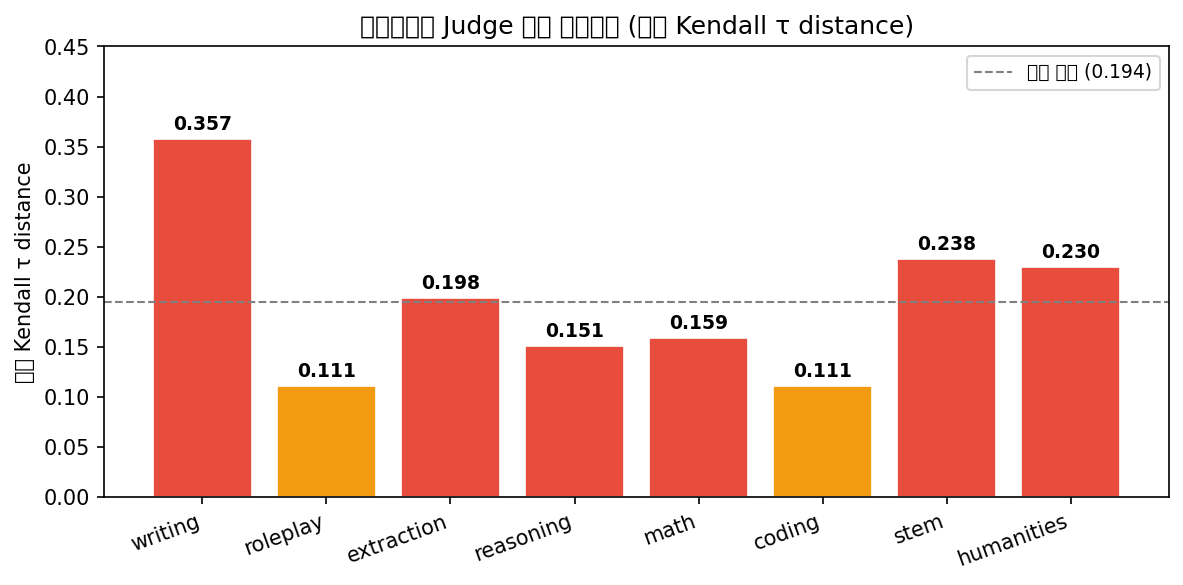
\includegraphics[width=\linewidth]{../figures/fig_category_tau.png}
  \caption{카테고리별 평균 Kendall $\tau$ distance.
  Writing이 0.191로 가장 높고, Coding이 0.083으로 가장 낮다.
  점선은 전체 평균(0.131).}
  \label{fig:cat_tau}
\end{figure}

\subsection{Judge 크기 스케일링과 불일치율}

Pairwise 불일치율은 Qwen-7B(78.75\%) $\to$ 14B(46.85\%) $\to$ 32B(32.86\%)로
단조 감소한다(그림~\ref{fig:scaling}). 그러나 불일치 쌍 내 first-position
승률은 84.2\%→93.5\%→94.9\%로 오히려 증가한다. \textbf{불일치율 감소가
곧 신뢰도 향상을 의미하지 않는다} — 남은 불일치가 더 강한 위치 편향 사례에
집중되기 때문이다. Bootstrap 95\% CI에서 7B--14B의 Spearman $\rho=0.821$,
14B--32B의 $\rho=0.750$으로 broad rank consistency는 유지되나, 순위 역전
구간이 존재한다.

\begin{figure}[t]
  \centering
  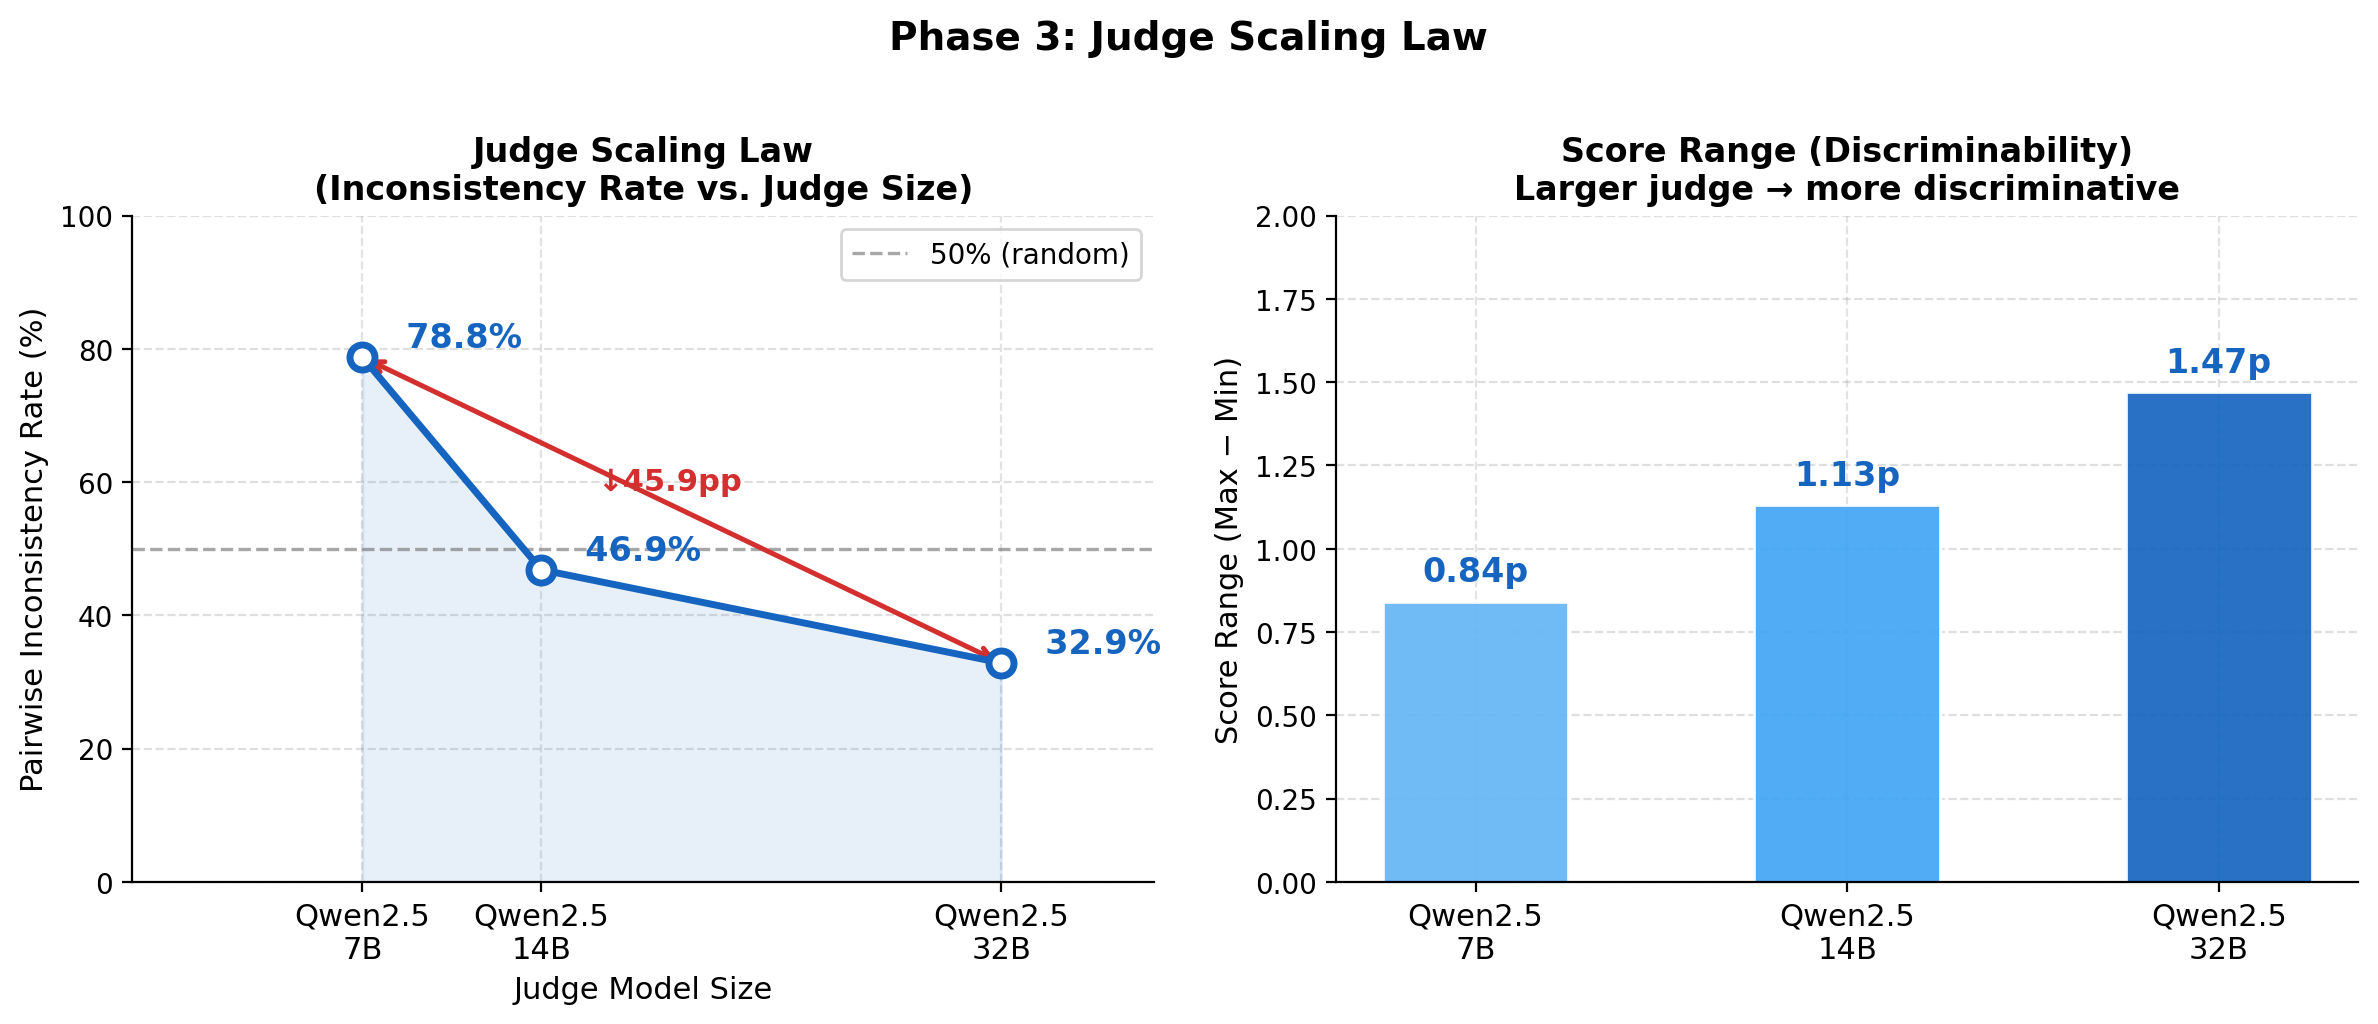
\includegraphics[width=0.95\linewidth]{../figures/fig4_judge_scaling.png}
  \caption{Qwen2.5 judge 크기별 pairwise 불일치율.
  단조 감소하나 불일치율만으로 신뢰도를 판단할 수 없다.}
  \label{fig:scaling}
\end{figure}

\subsection{Reference-guided 채점의 보정 효과}

그림~\ref{fig:ref_penalty}는 정답(reference)을 제공했을 때와 제공하지 않았을 때의
점수 차이를 보여준다. 모든 모델·모든 judge에서 reference 제공 시 점수가
하락한다. 평균 하락폭은 Qwen-7B $-1.2$점, Qwen-14B $-2.0$점,
Qwen-32B $-2.7$점, GPT-4o-mini $-2.6$점이다.

\textbf{소형 judge(7B)는 reference 없이도 관대하게 채점하지만, 대형 judge는
정답을 알았을 때 훨씬 가혹해진다.} 이는 소형 judge가 ``그럴듯해 보이는''
답변에 높은 점수를 주는 경향이 있음을 시사한다. 특히 Zephyr-7B-beta는
Qwen-7B에서 reference 없이 7.20점이지만 reference 제공 시 5.24점으로
1.96점 하락한다. 이 모델이 reference 기준으로는 실제로 낮은 품질임에도
소형 judge가 과대평가했음을 드러낸다.

\begin{figure}[t]
  \centering
  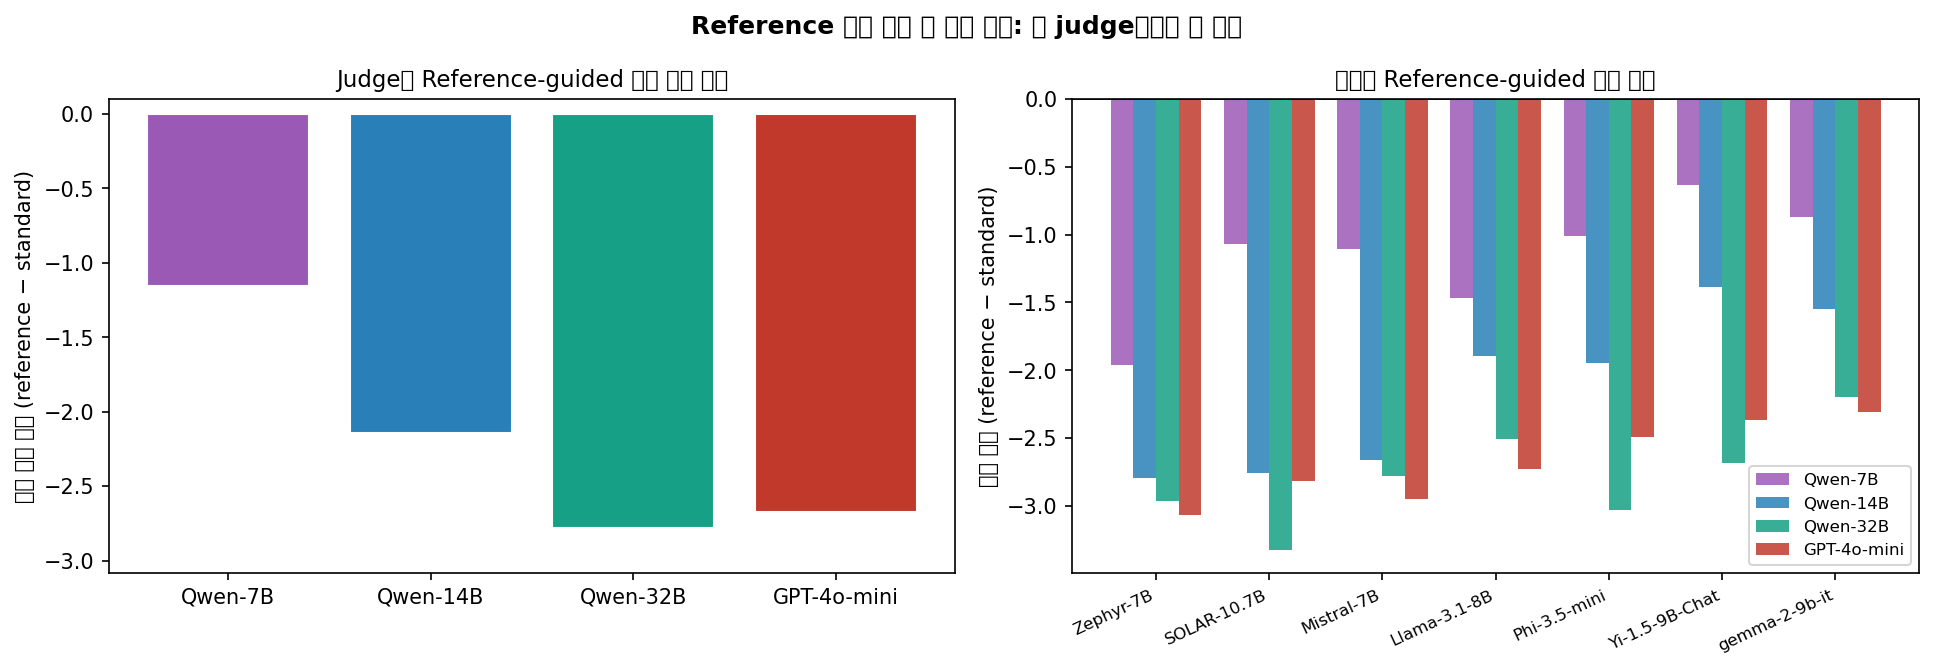
\includegraphics[width=\linewidth]{../figures/fig_reference_penalty.png}
  \caption{Judge별 Reference-guided 채점 시 점수 하락. 왼쪽: judge별 평균 하락폭.
  오른쪽: 모델별 judge별 하락폭. 큰 judge일수록 더 가혹하게 보정된다.}
  \label{fig:ref_penalty}
\end{figure}

\subsection{Turn 2 구조적 난이도}

카테고리별 Turn 1→Turn 2 점수 변화($\delta$)는 Reasoning($-0.89$)과
Math($-0.77$)에서 가장 크고, Writing($+0.12$)에서는 오히려 상승한다.
이는 MT-Bench Turn 2가 카테고리에 따라 구조적으로 난이도가 다름을 보여준다.
Reasoning·Math에서는 이전 답변을 이어받아 더 깊은 추론을 요구하므로
하락폭이 크고, Writing에서는 2nd turn의 수정·보완 요청이 오히려 모델에
유리하게 작용한다.

\subsection{tinyMT-Bench: 최소 변별 문항 세트}

문항별 변별도(모델 간 점수 표준편차)를 기준으로 상위 40문항(TopDisc-40)을
선택하면 전체 80문항과 Spearman $\rho=0.964$를 유지한다.
무작위 40문항 선택($\rho=0.750$ 평균) 대비 유의미하게 높으며,
11개 모델 풀 330개 hold-out split 반복 검증에서 60문항이 $\rho=0.998$의
안정적인 운영점임을 확인하였다. 이는 \textbf{평가 문항을 25\%로 줄여도
동일한 랭킹 신뢰도를 유지할 수 있음}을 의미한다.

% ─────────────────────────────────────────────────────
\section{결론}
% ─────────────────────────────────────────────────────

본 논문은 LLM-as-a-Judge에서 judge 선택이 모델 랭킹을 유의미하게 바꾼다는
것을 다각도로 실증하였다. 핵심 발견:
(1) judge 선택만으로 Kendall $\tau$ distance 최대 0.190의 랭킹 역전 발생
— 단일 judge 결과만으로 모델을 비교하는 것은 위험하다.
(2) 카테고리별 불안정성이 크게 다르다 — Writing(0.191)이
Coding(0.083)의 2.3배로, 주관적 카테고리에서 judge 의존성이 높다.
(3) 소형 judge는 정답 없이 관대하게 채점하지만, 대형 judge는
reference 제공 시 더 가혹하게 보정된다 — 점수 절댓값보다 상대 순위로
비교해야 하며, reference 유무를 명시해야 한다.
(4) Qwen2.5-32B는 GPT-4o-mini와 $\tau$ distance 0.048로 수렴하여
충분한 크기의 오픈소스 judge가 중립 reference를 대체할 수 있음을 보인다.
(5) TopDisc-40 문항 세트로 평가 비용을 절반으로 줄이면서 동일 랭킹 유지.

향후 연구로는 LLaMA 2 패밀리를 judge로 추가해 judge가 자기 패밀리 모델을
유리하게 채점하는 self-judge bias를 실증적으로 검증할 예정이다.

% ─────────────────────────────────────────────────────
\begin{thebibliography}{9}
\bibitem{zheng2023}
L. Zheng et al., ``Judging LLM-as-a-Judge with MT-Bench and Chatbot Arena,''
\textit{NeurIPS}, 2023.

\bibitem{shi2024}
J. Shi et al., ``Judging the Judges: A Systematic Investigation of Position Bias
in Pairwise Comparative Assessments by ChatGPT,''
\textit{arXiv:2406.07791}, 2024.

\bibitem{ye2024}
M. Ye et al., ``Justice or Prejudice? Quantifying Biases in LLM-as-a-Judge,''
\textit{arXiv:2410.02736}, 2024.

\bibitem{park2024}
S. Park et al., ``Prometheus 2: An Open Source Language Model Specialized in
Evaluating Other Language Models,''
\textit{arXiv:2405.01535}, 2024.
\end{thebibliography}

\end{document}
